\chapter{A rendszer implementálása}
A robot egy négykerekű kültéri mobilis robot $4W-SSMR$ amelynek négy különálló csiga áttétel, és egy DC motor mozgat.

\begin{table}[H]
\center
    \begin{tabular}{llll}
        \hline
        Paraméter               & érték     & Mértékegység     \\ \hline
        Szélesség               & 80        &   $[cm]$         \\
        Hosszúság               & 80        &   $[cm]$         \\
        Magasság                & 40        &   $[cm]$         \\
        Önsúly                  & 54        &   $[kg]$         \\
        Max sebessége           & 25        &   $[cm/s]$       \\
        Max fordulási sebesség  &25         &   $[\degree/s]$  \\
        Kerék-átmérő            &40         &   $[cm]$       \\
        Maximális 
        kerék forgatónyomaték   &1000       &   $[N/m]$        \\ 
    \end{tabular}
\end{table}

A roboton egy performáns számítógép felelős a ROSmaster és egyéb kiszolgáló nodok fűtatásáért, a rendszerhez, USB \ref{fig:CmodA7architektura} csatlakozóval kapcsolódó modulok:
\begin{table}[H]
\center
    \begin{tabular}{llll}
        \hline
        Modulnév            & Leírás     \\ \hline
        2xFPGA                          &   \multicolumn{2}{p{12cm}|}{\raggedright CmodA7 $https://reference.digilentinc.com/reference/programmable-logic/cmod-a7/reference-manual$ }      \\
        IMU                       &   \multicolumn{2}{p{12cm}|}{\raggedright ESP8266 arduino alapú rendszer,
        SPI protokollon keresztül olvassa az IMU mert értékeit,
        átalakítás után string formában uart protokollon
        küldődik a kiszolgáló ROS nodnak }       \\
        GPS                     &  \multicolumn{2}{p{12cm}|}{\raggedright Uart porton NMEA protokoll alapján
        ROS node fogadja az értékeket. }        \\
        LIDAR                          & \multicolumn{2}{p{12cm}|}{\raggedright Leírás:
        $https://www.robotshop.com/media/files/pdf2/rpk-02-datasheet.pdf$,
        gyártó által biztosított ROS
        $http://wiki.ros.org/rplidar$
        integráció.     }   \\
       
    \end{tabular}
\end{table}



%\lhead{Modulok es kapcsolatok}

\section{Alacsony szintu modulok} 

A roboton alacsonyszintű feladatait amelyek a motor hajtásokhoz kapcsolódó szenzorokat és vezérlő jelek elő allitasara hivatott a kétdaram CmodA7 20T FPGA fejlesztőlap. Négy tengely szogsebesseget kel szabályozni, egy FPGA két hajtást valósít meg. A \ref{fig:CmodA7architektura} alapján egy hajtáshoz tartozó I/O-k:

\begin{table}[H]
\center
\begin{tabular}{lll}
\hline Név                            & Darab              & Típus  \\ \hline
Inkrementális enkoder           & 2           & Digitális Input \\
Árammérő szenzor                & 1                  & Analóg Input \\
Motor vezérlő                   & 3                  & Digitális Output \\
Végálas kapcsoló                 & 1                  & Digitális Input        
\end{tabular}
\end{table}




\renewcommand{\img}{SajatRobot/SzerkAbrak/cmoda7modulok.jpg}
\renewcommand{\sources}{*}
\renewcommand{\captionn}{CmodA7 FPGA-ban kialakított architektúra amely a szenzorok és motor hajtások kezelésre hivatott }
\renewcommand{\figlabel}{CmodA7architektura}
\begin{kep}
\begin{figure}[H]
\centering
\ifthenelse{\equal{\svg}{*}}
{
    \includegraphics[width=\aspectratioPic\textwidth,angle=\rotationAnglePic]{\img}
}
{
    \includesvg[width=\aspectratioPic\textwidth,angle=\rotationAnglePic]{\img}
}

 \ifthenelse{\equal{\sources}{*}}
    { \captionof{figure}{ \captionn}}
    { \captionof{figure}{ \mand{\mand{\captionn}{Forrás:}}{}} }
  	

\ifthenelse{\equal{\figlabel}{*}}
    {}
    {\label{fig:\figlabel}}%
    
\renewcommand{\figlabel}{*}



\end{figure}
\end{kep}
\renewcommand{\aspectratioPic}{1}
\renewcommand{\rotationAnglePic}{0}
\renewcommand{\svg}{*}


A rendszer tervezesenel a fo koncepcio az volt hogy a rendszer arhitekturaja dinamikus legyen a fejleszhetoseget tekitve, igy a \ref{fig:CmodA7architektura} levo arhitekurat kaptuk. 


\renewcommand{\img}{SajatRobot/FPGAmodulok/uBlazeAndFpgaUML.jpg}
\renewcommand{\sources}{*}
\renewcommand{\captionn}{MicroBlaze proceszoron futo szoftver diagramja}
\renewcommand{\figlabel}{MicroblazeSoft}
\begin{kep}
\begin{figure}[H]
\centering
\ifthenelse{\equal{\svg}{*}}
{
    \includegraphics[width=\aspectratioPic\textwidth,angle=\rotationAnglePic]{\img}
}
{
    \includesvg[width=\aspectratioPic\textwidth,angle=\rotationAnglePic]{\img}
}

 \ifthenelse{\equal{\sources}{*}}
    { \captionof{figure}{ \captionn}}
    { \captionof{figure}{ \mand{\mand{\captionn}{Forrás:}}{}} }
  	

\ifthenelse{\equal{\figlabel}{*}}
    {}
    {\label{fig:\figlabel}}%
    
\renewcommand{\figlabel}{*}



\end{figure}
\end{kep}
\renewcommand{\aspectratioPic}{1}
\renewcommand{\rotationAnglePic}{0}
\renewcommand{\svg}{*}





\subsection{FPGA alapu uart komunikacio}
\label{FPGAcomuSection}
Megvalositva a komunikaciot a kiszolgalo ROS noddal, amely UART protokolra epitett sajat uzenetekbol all \ref{fig:FPGAComCsomagAlt}.

\renewcommand{\img}{SajatRobot/FPGAmodulok/ProtokolDiagram.jpg}
\renewcommand{\sources}{*}
\renewcommand{\captionn}{FPGA komunikacios protokol altalanos csomag szerkezet}
\renewcommand{\figlabel}{FPGAComCsomagAlt}
\begin{kep}
\begin{figure}[H]
\centering
\ifthenelse{\equal{\svg}{*}}
{
    \includegraphics[width=\aspectratioPic\textwidth,angle=\rotationAnglePic]{\img}
}
{
    \includesvg[width=\aspectratioPic\textwidth,angle=\rotationAnglePic]{\img}
}

 \ifthenelse{\equal{\sources}{*}}
    { \captionof{figure}{ \captionn}}
    { \captionof{figure}{ \mand{\mand{\captionn}{Forrás:}}{}} }
  	

\ifthenelse{\equal{\figlabel}{*}}
    {}
    {\label{fig:\figlabel}}%
    
\renewcommand{\figlabel}{*}



\end{figure}
\end{kep}
\renewcommand{\aspectratioPic}{1}
\renewcommand{\rotationAnglePic}{0}
\renewcommand{\svg}{*}



A modul megvalositja mindet iranyban a keretezest, parameterkent atadhato egy-egy karaketr jelzi az uzenet kezdetet es veget jelen esetben az $S$ csomag kezdetet, mig a $P$ a csomag veget jelzik.
A proceszor cimtartomanyaba ilesztet modul rendelkezik egy 400byte karakterbol allo memoriaval, amelyhez egyidoban a proceszor es a hardver is hozaferhet \cite{DualPortRam}.
A kezdo keret beerkezte utan minden karakter bekerul a 400byte hoszu memoriaba sorba, kivetelt kepez ezalol a binaris adat tomb ahol a skip\footnote{specialis karakterek amelyek jelzik az ertelmezo szamara hogy olyan karakter kovetkezik amelyet a protokol ertelmezeseben nem kell vegrehajtani.} karakterek kikerulnek a tombol.Jelen esetben a \{ es \} kozt levo karakterek nem kerulnek ertelmezesre. A \{ utani elso karakter megadja a binaris adat hoszat igy tudja az ertelmezo hogy hol kell varnia a lezaro karaktert.

\subsection{Paramterek FPGA modul}
% Please add the following required packages to your document preamble:
% \usepackage{multirow}
% \usepackage[normalem]{ulem}
% \useunder{\uline}{\ul}{}

\begin{table}[H]
\begin{tabular}{lllllp{6cm}}
\hline \multirow{2}{*}{Id} & \multirow{2}{*}{\begin{tabular}[c]{@{}l@{}}Nev \\ (X lehet A vagy B)\end{tabular}} & \multicolumn{2}{l}{Ertekek} & \multirow{2}{*}{Tipus} & \multirow{2}{*}{Leiras}                                                                                                                      \\
                    &                                                                                    & Min         & Max           &                        &                                                                                                                                              \\ \hline
1                   & TsTimerPeriod                                                                      & 1           & 1000          & int16                  &  Mintavetelezesi periodus {[}ms{]} ban.                                                                                                      \\
2                   & GetDataPeriodical                                                                  & 0           & 1             & int16                  &  Kapcsolo ha 0 akkor nem kuld az FPGA mert ertekeket, kulomben a TsTimerPeriod periodusi mintavetellel kuld.                                  \\
3                   & TorqueCoefX                                                                        &             &               & float16                &  Motor aram es nyomatek kozti egyuthato.                                                                                                      \\
4                   & ActiveControllerX                                                                  & 0           & 65535         & int16                  &  Valaszhato szabalyzo tipusok hajtasonkent 0=Szoftvare PID szogsebesseg, 1=Hardver PID szogsebesseg, 2=Szoftver PID aram, 3=Hardver PID aram  \\
5                   & MaxControlSiggnalX                                                                 & 0           & 32760         & sint16                 &  A beavatkozo PWM jel maximalis kitoltesi tenyezoje, linearisan 0-\textgreater{}0\% -tol 32760-\textgreater{}100\% -ig.                       \\
6                   & IncSenzResX                                                                        & 0           & 65535         & int16                  &  Inkrementalis szenzor altal generalt inpulzusok szama egy teljes kerekfordulatra.FPGA oldalon ez a szam 10-el szorzodik.                     \\
7                   & IncSenzCountDirectionX                                                             & -1          & 1             & sint16                 &  inkrementalis szenzor jeleit feldogozo mudul szamolasi iranyanak valtoztatasara szolgalo egyuthato.                                          \\
8                   & Kp\_Whell\_PidX                                                                    & 0           &               & float16                &  szogsebeseg szabalyzo, PID erositesi parametere.                                                                                             \\
9                   & Ti\_Whell\_PidX                                                                    &             &               & float16                &  szogsebeseg szabalyzo, PID integralasi ido.                                                                                                  \\
10                  & Td\_Whell\_PidX                                                                    &             &               & float16                &  szogsebeseg szabalyzo, PID derivalasi ido.                                                                                                   
\end{tabular}
\end{table}


\renewcommand{\img}{SajatRobot/FPGAmodulok/UartUML.jpg}
\renewcommand{\sources}{*}
\renewcommand{\captionn}{FPGA hardver/MicroBlaze proceszor es ROS node kozti komunikacio megvalistiasa UART protokol alapjan }
\renewcommand{\figlabel}{FPGAuartRos}
\begin{kep}
\begin{figure}[H]
\centering
\ifthenelse{\equal{\svg}{*}}
{
    \includegraphics[width=\aspectratioPic\textwidth,angle=\rotationAnglePic]{\img}
}
{
    \includesvg[width=\aspectratioPic\textwidth,angle=\rotationAnglePic]{\img}
}

 \ifthenelse{\equal{\sources}{*}}
    { \captionof{figure}{ \captionn}}
    { \captionof{figure}{ \mand{\mand{\captionn}{Forrás:}}{}} }
  	

\ifthenelse{\equal{\figlabel}{*}}
    {}
    {\label{fig:\figlabel}}%
    
\renewcommand{\figlabel}{*}



\end{figure}
\end{kep}
\renewcommand{\aspectratioPic}{1}
\renewcommand{\rotationAnglePic}{0}
\renewcommand{\svg}{*}



Az uzenet veget jelzo karakter az \ref{fig:FPGAuartRos} lathato folyamat alapjan a modul general egy hardveres megszakitast a procesornak, a proceszor kiolvassa az adat kezdocimet, es elkezdi kiolvasni az adatokat a sajat adatmemoriajaba. Ekozben ha uj csomag erkezik a hardver komunikacios modulhoz, elkezdodik annak beirasa a memoriaba, az elozo adatok felulnemirasaval. A megszakitas ertelemzi a csomag tipusat es annak megfeleloen vegrehajtja a muveleteket amelyek lehetnek: Parameter ertekenek a bealitasa,  Parameter ertekenek a lekerdezese, eloirt ertekek fogadasa, mert erteke kuldese, ACK megerosito uzenet kuldese/fogadasa.

Az uzenetek kuldese hasonlokepen mukodik az olvasashoz, a hardver megoldja a keretezest es a skip karakterek beszurasat is.




\subsubsection{Kommunikáció sebessége}

Az uart sebesege 1MBd \footnote{megabaud} ami megfelel 131072 byte/s adatforgalomnak. A valosagban a komunikacio hibatlanul mukodik 1ms periodussal kuldott 100byte hoszu uzeneteket.

\begin{equation}
    frekvencia = \frac{131072}{SizeOfPachage}=\frac{131072[byte/s]}{100[byte]}=1310,072 [Hz]
\end{equation}

\subsubsection{Biztonsagi megoldasok}

Abbana az esetben ha kikultuk az elirt ertekeket a modulnak es ezutan a komunikacio megszakadt a modullal akkor a szabalyzok probaljak tartani az elirt erteket annak elenere is hogy az mar lehet hogy megkelet volna valtozzon. Erre a celra bepitesre kerult egy uzenet es egy logika (HeartBeat) amely csak a komunikacios modulhoz erkezik meg, es jelzi hogy a ROS jolmukodik, es forditva is.Abban az esetben ha a komunikacio megszakad lealitja a motrokat es a szabalyzokat,  \ref{fig:FPGAuartRos} alapjan az Enable(EN) jel.

\begin{table}[H]
\center
\begin{tabular}{lll}
\hline Irany   & Uzenet & Periodis    \\ \hline
FPGA->ROS &  SEP        & 300 ms kotelezo         \\
ROS->FPGA &  mintavetelezett ertekek kuldese & dinamikusan modosithato                   
\end{tabular}
\end{table}
















\newpage
%\lhead{ROS sajat robot}

\section{ROS}

A robot irányítását megtehetjük azáltal, hogy csatlakozunk wifin keresztül a robothoz. Az irányításhoz szükséges egy számítógép, amelyre telepítve kell  legyen a ROS. A kliens gépen fognak futni a következő felhasználói eszközök:
-a rendszerben futó programok által loggolt üzeneteket szűrhetjük és tekinthetjük meg valós időben.
-a paramétereket bealíthatjuk egy grafikus felhasználói felület segítségével ($dinamic\_reconfigure$).-rviz amelyel megjeleniti a robot 3D modelljét a térképen, a robot aktuális pozíciójában és irányában a környezetéhez viszonyítva.
-$JuglerPlot$ segítségével online ábrázolhatunk mért értékeket mint pl.: a szabályzókörökben mért értékeket.

Jelenleg két működési mód közül választhatunk:

	-távirányítóról vezérelve. A távirányítón található egy joystick, amely segítségével a robotnak referencia sebességeket írhatunk elő. A hozzárendelt referencia rendszerhez képest az X tengelyen m/s sebességet adunk meg, míg a Z tengelye körül \degree/s forgási sebességet adunk meg.
A távirányító két gomb folyamatosan lenyomva tartásával a deadman kapcsolót valósíthatjuk meg. Abban az esetben, ha a két gomb nincsen lenyomva, a szabályzók működése és a pwm generátorok kimenete letiltva marad.

	-automata mód, itt rviz program segítségével előírhatunk egy referencia pozíciót és irányt ahova szeretnénk, hogy a robot eljusson. Ez alatt a távirányítón a deadman kapcsolókat lenyomva kell tartanunk. A referencia értékeket megadhatjuk rviz használata nélkül azáltal, hogy a megfelelő típusú és nevű üzenetet beküldjük a ROS rendszerbe.



\begin{figure}[H]
  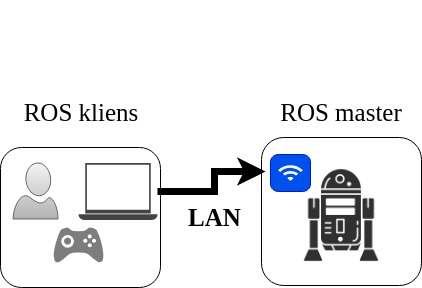
\includegraphics{tikz/RobotUserLan.jpg}
  \caption{Robothoz csatlakozás a Wifi-n keresztül.}
  \label{fig:RobotUserLan}
\end{figure}


Az \ref{fig:ROSgraph} láthatóak a főbb nodok, topikok és a köztük levő relációk. A nodok és a topikok leírását a \ref{Tab:nodok}

\begin{table}[H]
\centering
\begin{tabular}{lp{3cm}p{8cm}}
\hline Node Név & Típus & Leírás \\ \hline
  /R és /L      &  FPGA
  Communication
  Modul     &  Az FPGA-val való kommunikációért felelős. Adatokat fogad/küld  a \ref{FPGAcomuSection} fejezetben leírt protokoll alapján, amelyeket továbbít a ROS operációs rendszerben működő nodoknak.     \\
  /ImuInBoxA       &    Imuxxxx   &  Feladata szöveges formában érkező adatok feldolgozása és a ROS keretrendszerbe integrálását oldja meg. Mért fizikai mennyiségek:       \\
  /WheelOdometry       &       &   Kerekek mozgásából számolt robot elméleti pozíciója a térben     \\
  /TeleopJot      &       & Feladata a joystick-től érkező parancsok fogadása. Megvalósítja a $Dead Man Switch$ gomb kezelését, létrehoz egy globálisan engedélyező jelet a /setEMS-t és a /TeleopSig-t, amely előírja a robot lineáris mozgási sebességét és a forgási sebességét a Z tengely körül.  \\
  /rplidarNode & & A lidar mérési adatait olvassa ki és továbbítja a /scan topikban.\\
  /rosserial\_server & & A megvalósítja a kommunikációt egy esp8266 fejlesztőlap és a ROS között, amely az akkumulátorok feszültségeinek a merését végzi \cite{RosSerial}.\\
  /Joy & & Joystick eszközök integrációját valósítja meg \cite{rosjoy}.\\
  /hector\_mapping & & Lidar mérései alapján 2D térképet készit a környezetről, miközben lokalizálja a robotot ezen a térképen \cite{roshectormap}\\
  /Measurement & & mérésék elvégzésére szolgáló node, amely egy élőre beállított intervallumokban a megadott referencia értékeket küld ki az FPGA ban levő szabályzóknak.\\
  /TelepoController & & Átalakítja a robot sebesség állapotait és kiszámolja nyílt hurokban a szabályzok előírt értékeit. Abban az esetben, ha a /movebase nodot használjuk, ez megoldja a robot pozíció szabályozását a térképen, így a $/cmd_vel$ csomagot csak átalakítja /refVals csomaggá azáltal, hogy azonos oldalon levő kereke ugyanazt a referencia értéket kell követniük.
  
\end{tabular}
 \label{Tab:nodok} 
\end{table}

\subsection{Üzenet típusok (.msg)}
Az alábbi táblázatban láthatjuk a ROS operációs rendszer által szolgáltatott .msg üzenetek kiterjesztését, amelyek lehetővé teszik az FPGA integrációját a ROS környezethez.
\begin{table}[H]
\centering
\begin{tabular}{lllp{6cm}}
\hline \textbf{Üzenet típus}              & \textbf{Értékek}   & \textbf{Erkek típusa} & \textbf{Leírás} \\ \hline
 header                   &     -     &      std\_msgs/Header      &   Minden üzenet tartalmaz egy fejlécet, amely információkat tartalmaz az üzenetről. \\   
                          & seq       &      uint32        &   minden üzenetet egyedileg beazonosító szám     \\
                          & stamp     &      time        &  idő-bélyeg amely a küldés idő-pillanatát tárolja.      \\
                          & frame\_id  &      string        &        \\  \hline
                          
\hline  \multirow{1}{*}{/GlobalEnable}  &   systemIsOk        &    int16          &    
                                                                          =0 - a HLC működik.
                                                                          
                                                                          <>0 -  a HLC nem nem működik      \\    \hline                    
\hline\multirow{4}{*}{/refVals} & names     & string{[}{]} &        \\
                          & ref\_position  & float{[}{]}  & előírt szög pozíció       \\
                          & ref\_velocity & float{[}{]}  &  előírt szög sebesség      \\ 
                          & ref\_effort &    float{[}{]}  &  előírt forgatónyomaték    \\\hline
 \hline \multirow{1}{*}{/setEMS}  &   value        &     int16         &      =0 - Vészleállító aktív.
                                                                          
                                                                       <>0 -  Vészleállító nem aktív  \\     \hline 
\hline\multirow{3}{*}{/joyControll} & vx     & float64 &    A robot X tengely mentén előírt sebessége m/s-ban.    \\
                          & omega  & float64  & előírt szög pozíció   A robot Z tengely körüli forgása \degree/s-ban.    \\
                          & ControlMode & int64  &  Választhatunk a HLC szabályzok típusa vagy a manuális irányítás közül 
                           =0 move\_base szabályzó, =1 manuális irányítás joystick segítségével.\\   \hline                                                                       
\end{tabular}
\end{table}

A \ref{fig:ROSgraph} ábrán láthatjuk a nodok és az üzenetek közti kapcsolatot.

\renewcommand{\img}{SajatRobot/ROS/rosgraph.svg}
\renewcommand{\sources}{*}
\renewcommand{\svg}{svg}
\renewcommand{\aspectratioPic}{1.4}
\renewcommand{\rotationAnglePic}{90}
\renewcommand{\captionn}{ROS graph}
\renewcommand{\figlabel}{ROSgraph}
\begin{kep}
\begin{figure}[H]
\centering
\ifthenelse{\equal{\svg}{*}}
{
    \includegraphics[width=\aspectratioPic\textwidth,angle=\rotationAnglePic]{\img}
}
{
    \includesvg[width=\aspectratioPic\textwidth,angle=\rotationAnglePic]{\img}
}

 \ifthenelse{\equal{\sources}{*}}
    { \captionof{figure}{ \captionn}}
    { \captionof{figure}{ \mand{\mand{\captionn}{Forrás:}}{}} }
  	

\ifthenelse{\equal{\figlabel}{*}}
    {}
    {\label{fig:\figlabel}}%
    
\renewcommand{\figlabel}{*}



\end{figure}
\end{kep}
\renewcommand{\aspectratioPic}{1}
\renewcommand{\rotationAnglePic}{0}
\renewcommand{\svg}{*}


\subsection{FPGA kommunikációs modul ROS oldali integració}

A ROS biztosít a fejlesztőknek egy megoldást, amelyek képesek újonnan létrehozott robot integrálását ROS környezetben \cite{RosSerial}. Előnye hogy gyorsan látványos eredményt érhetünk el, de a működés sebességben és az üzenetek méretében is korlátozott. Ezen hátrányokból kifolyólag sajátos integráció szükséges, amely integrálta az FPGA UART kommunikáció protokollt a ROS keretrendszerben működő más modulokhoz.

A \ref{fig:ROStoUart} diagramon a kommunikáció node technikai megvalósítását láthatjuk. Különálló szál gondoskodik az UART adatok olvasasáról és írásáról. Az üzenetek értelemezését egy külön szál végzi és hívja fel a kiszolgáló függvényeket.
A paraméterek helyes beállításáról a ParamThread szál gondoskodik, paraméterek helyes beállításáról FPGA oldalon. Abban az esetben, ha a hardver kap egy űj paramétert a \ref{fig:MicroblazeSoft} alapján az FPGA visszaküldi a kapott paramétert, a visszajelzésből eldönthető, hogy a paraméter  a hardverben helyesen állítódott e be. Abban az esetben, ha nem megfelelő, újraküldődik mindaddig amíg nem sikeres a beállítás.

A paraméterek kezelésére a ROS paraméter szerver a felelős \cite{parameterserver}, abban az esetben, ha egy paraméter megváltozott, amely az illető nodehoz köthető, akkor a \ref{fig:ROStoUart} ábrán látható ParameterValtozott esemény előidézi a  megváltozott paraméter értékének az elküldését  FPGAnak irányába.

A globális engedélyező jel a \ref{fig:ROStoUart} MasterLive Enable,  /globalEnable típusú üzenettel engedélyezhetjük a szabályzok működését, a folyamatos működéshez 500ms periódussal kell érkeznie. Abban az esetben, ha a központi számítógép valami okból leállna, akkor a hardveres szabályzok is leállnak. A node 300ms periódussal küldi tovább az engedélyező jelet az FPGA modulnak. A HardverLive jel információt szolgáltat a többi ROS környezetben futó és a működés szempontjából kritikus nodenak, hogy az adott modul megfelelően működik e. Ezen információ birtokában a HeartBeat node leállítja a rendszert, ha egyik FPGA modul nem válaszol.

\renewcommand{\img}{SajatRobot/ROS/NodeUML.jpg}
\renewcommand{\sources}{*}
\renewcommand{\captionn}{ROS integrálása Uart protokolhoz.}
\renewcommand{\figlabel}{ROStoUart}
\begin{kep}
\begin{figure}[H]
\centering
\ifthenelse{\equal{\svg}{*}}
{
    \includegraphics[width=\aspectratioPic\textwidth,angle=\rotationAnglePic]{\img}
}
{
    \includesvg[width=\aspectratioPic\textwidth,angle=\rotationAnglePic]{\img}
}

 \ifthenelse{\equal{\sources}{*}}
    { \captionof{figure}{ \captionn}}
    { \captionof{figure}{ \mand{\mand{\captionn}{Forrás:}}{}} }
  	

\ifthenelse{\equal{\figlabel}{*}}
    {}
    {\label{fig:\figlabel}}%
    
\renewcommand{\figlabel}{*}



\end{figure}
\end{kep}
\renewcommand{\aspectratioPic}{1}
\renewcommand{\rotationAnglePic}{0}
\renewcommand{\svg}{*}


\subsection{Előirt értékek}
A /refVals típusú üzenetben megadjuk minden egyes motor előírt értékét annak fövenyében $\degree/s$ hogy sebesség alapján szabályzunk vagy $N/m$ előírt nyomaték alapján.


\subsection{Vonatkoztatási Rendszerek }
A  vonatkoztatási rendszerek szükségesek, mert a szenzorok és beavatkozó eszközök egymáshoz viszonyított helyzete és poziciója is változhat. Sok esetben szükséges ismernünk egy adott eszköznek a múltbeli helyzetét, vagy egy másik vonatkoztatási rendszerhez képest a pozícióját vagy irányát. A ROS biztosít egy tf \cite{rosTF} nevű csomagot amely megvalósítja a szűkséges transzformálásokat a $VNR$-k között. 
A \ref{fig:ROSframes} látható a kialakított vonatkoztatási rendszerek a roboton amely hűen modellezi a fizikai robot kialakítását.
A vonatkoztatási rendszereket két csoportba oszthatók:

\begin{enumerate}[label=(\alph*)]
\item rögzített pozíció és szögek, szabadságok 0:
Szenzorok laser, BODY\_link, wheel\_odom, ImuALink VNR je a base\_link a globális robot VNR hoz:
\item rögzített pozíció csak szögek változnak, szabadságok 1: Kerekek VNR je: FL\_link, BL\_link, FR\_link, BR\_link a BODY\_link hez képest csak Y körül foroghat.
\item pozíció és szög is változik, szabadságok 6:
A robot base\_link az helymeghatározás odom, és az odometria a térképhez map viszonyítva.
\end{enumerate}


A robot modellt ROS környezetben URDF robot leíró, xml alapú fájlal tehetjük meg, \cite{rosURDF}
\cite{rosJoint} \cite{rosLink}.
Az <origin> tag az xzy paraméter alatt, megadhatjuk a csukló pozícióját mindhárom tengelyen, méterben kifejezve a <parent> tagban szereplő linkhez képest. Az rpy paraméter alatt az elfordulásokat rendre x, y, z tengelyek mentén radiánban kifejezve.
Az <axis> tagban beállíthatjuk a kényszereket, jelen esetben csak az y tengely körüli forgás engedélyezett, azaz a kerekek esetében. 
Az <link> tagban robot elemeket hozhatunk létre. Az alábbi XML-ben látható a robot fizikai leírása, amely megfelel a valós szerkezetnek.
\begin{lstlisting}[language=XML]
<robot name="mobile_robot_platform_4Wheel">
	<link name="base_link" > </link>
	<link name="FL_link" > </link>
	<link name="BR_link" > </link>
	<link name="BL_link" > </link>
	<link name="BODY_link"> </link>  
	<link name="ImuALink"> </link>  
	<link name="laser"> </link> 

	<joint name="FL" type="continuous">
		<parent link="BODY_link"/>
		<child link="FL_link"/>    
		<origin xyz="0.29 -0.33 0" rpy="0 0 0" />
		<axis xyz="0 1 0" />
	</joint>

	<joint name="FR" type="continuous">
		<parent link="BODY_link"/>
		<child link="FR_link"/>    
		<origin xyz="0.29 0.330 0" rpy="0 0 0" />
		<axis xyz="0 1 0" />
	</joint>

	<joint name="BL" type="continuous">
		<parent link="BODY_link"/>
		<child link="BL_link"/>
		<origin xyz="-0.29 -0.330 0" rpy="0 0 0" />
		<axis xyz="0 1 0" />
	</joint>

	<joint name="BR" type="continuous">
		<parent link="BODY_link"/>
		<child link="BR_link"/>     
		<origin xyz="-0.29 0.330 0" rpy="0 0 0" />
		<axis xyz="0 1 0"/>
	</joint>

	<joint name="imuAandGPS" type="fixed">
		<parent link="base_link"/>
		<child link="ImuALink"/>
		<origin xyz="0.125 0.03 0.11" rpy="0 0 0" />
	</joint>

	<joint name="laserAJoin" type="fixed">
		<parent link="base_link"/>
		<child link="laser"/>
		<origin xyz="0.39 -0.02 0.23" rpy="0 0 3.14" />
	</joint>  

	<joint name="contact" type="fixed">
		<parent link="base_link"/>
		<child link="BODY_link"/>
	</joint> 
</robot>
\end{lstlisting}

A \ref{fig:ROSframes} láthatjuk, hogy a robot törzsét a $BODY\_link$ alkotja, amelyhez kapcsolódnak a kerekek: $BL\_link,FL\_link,BR\_link,FR\_link$. A $base\_link$ és a $BODY\_link$ egybe esnek. A szenzorok a $laser$, amely a lidarnak felel meg, $ImuALink$ IMU szenzor ezek a $base\_link$-hez kapcsolódnak.
A $map$ VNR a térképnek, amelyen meghatározzuk a robot pozícióját $odom$.

\renewcommand{\img}{SajatRobot/ROS/frames.svg}
\renewcommand{\sources}{*}
\renewcommand{\svg}{svg}
\renewcommand{\aspectratioPic}{1.5}
\renewcommand{\rotationAnglePic}{90}
\renewcommand{\captionn}{A megvalósított robot VNR-k közti reláció }
\renewcommand{\figlabel}{ROSframes}
\begin{kep}
\begin{figure}[H]
\centering
\ifthenelse{\equal{\svg}{*}}
{
    \includegraphics[width=\aspectratioPic\textwidth,angle=\rotationAnglePic]{\img}
}
{
    \includesvg[width=\aspectratioPic\textwidth,angle=\rotationAnglePic]{\img}
}

 \ifthenelse{\equal{\sources}{*}}
    { \captionof{figure}{ \captionn}}
    { \captionof{figure}{ \mand{\mand{\captionn}{Forrás:}}{}} }
  	

\ifthenelse{\equal{\figlabel}{*}}
    {}
    {\label{fig:\figlabel}}%
    
\renewcommand{\figlabel}{*}



\end{figure}
\end{kep}
\renewcommand{\aspectratioPic}{1}
\renewcommand{\rotationAnglePic}{0}
\renewcommand{\svg}{*}



\section{Kerekek Pid Szabalyzo hangolas}

A pid, a legelterjedtebb szabályozó egyszerű feladatok elvégzésére, esetünkben is elegendő a kerekek szögsebesség szabályzására kerekenkénti egy PID szabályzóval. A PID szoftveresen fut a uBlaze processzoron. Bemenete egy előírt forgási sebesség \degree/s ban és kimenete egy -32000 és 32000 egész típusú értek. A kimenti érteke a PWM kitöltési tényezőt jeleni, az előjel pedig a beavatkozás irányát.
Matlab/Simulink környezetben használva a Robotix Toolbox segítségével direkben pwm beavatkozo referenica erteket irtam elo a motroknak. A beavatkozó jel előállítása és elküldési a fizikai eszköznek 0-100\%-ig 10\% lépcsőkben amelyek 0\% kitoltesekkel vanak megszakitva. A mert adatokat rosbag csomagba mentve majd a System Identification Toolbox használatával identifikáljuk a rendszer modellt. A rendszer bemenete egy beavatkozójel ami fizikailag feszültségnek fele meg 0V és 12V között. A kimenetek a forgási sebesseg.
A mert adatokat Matlab/System Identification hasznalataval megbecsuljuk a rendszer modeleket. Nemlinearis modelt becslunk 
Hammerstein-Wiener model \cite{matlabhwmmodel} hasznalva, 1 kimenet es 1 bemenet, a linearis atviteli fugveny fokszama:
zerusok nb = 2, polusok nf = 3, keses a bemenet es a kimenet kozott nk = 1. A becsult adatok 94\% ban megfelelnek a mert rendszernek.          

A mereseket a robot kerekei es a talaj erintekzese nelkul vegeztem.
A becsult modelt a bemenet 50/\%  korul linearizaljuk es a linearizalt modelbol atviteli fugvenyt kesztunk. 
$tf = tf(linearize(model,16000));$ utasutast hasznalva Matlab kornyezetben. A linearizalt modelt Matlab/PidTuning eszkozt hasznalva behangolunk kiszamitjuk a megfelelo PID szabalyzo parametereit.


\tikzstyle{block} = [draw, fill=white, rectangle, 
    minimum height=3em, minimum width=6em]
\tikzstyle{sum} = [draw, fill=white, circle, node distance=1cm]
\tikzstyle{matlab} = [draw, fill=white, circle, node distance=1cm]
\tikzstyle{input} = [coordinate]
\tikzstyle{output} = [coordinate]
\tikzstyle{pinstyle} = [pin edge={to-,thin,black}]
\begin{center}
\begin{tikzpicture}[auto, node distance=2cm,>=latex']

   \node [block] (matlab) {Matlab/Simulink};
   \node [block, right of=matlab, node distance=4cm] (system) {System};
   \node [block, below of=system] (rosbag) {ROS bag};

    \node [right of=matlab,fill=black,inner sep=1.2pt,node distance=62] (umid) {};
    \draw [->] (matlab) -- (system);
%---------------- 
    \path (system.north east)--(system.south east) foreach \j in {1,...,2} {%
        coordinate [pos=1/3*\j] (z\j)
    };
    
    \foreach \i/\name/\nameNode/\text  in {1/{Omega}/{Om}/{$    \Omega$},2/{Current}/{Cu}/{I}}
    {  
        \node [output, right of=system, node distance=\i*15] (\nameNode) at (z\i) {};
        \node [fill=black,inner sep=1.2pt, right of=system, node distance=\i*15] (\nameNode) at (z\i) {};
        \node [output, right of=system, node distance=0] (\nameNode1) at (z\i) {};
        \node [output, right of=system, node distance=50] (\nameNode2) at (z\i) {};
        \draw [->] (\nameNode1) -- node[name=eu1,right of=Om2,node distance=33] {\text} (\nameNode2);
    }


%----------------
    \path (rosbag.north east)--(rosbag.south east) foreach \k in {1,...,2} {%
        coordinate [pos=1/3*\k] (z\k)
    };
    \foreach \i/\name  in {1/{inRbagOmeg},2/{inRbagCur}}
    {  
        \node [input, left of=rosbag, node distance=1.5] (\name) at (z\i) {};
    }
    

    \draw [<-] (inRbagCur) -| (Cu); crossing over
    \draw [<-] (inRbagOmeg) -| (Om);
    \draw [->] (umid) |-(rosbag);
    
\end{tikzpicture}
\end{center}

A becsült rendszer átviteli függvénye $H_s(z)$, mintavetelezesi periódus Ts: = 0.05s.

\subsection*{Nagyobik fokozatban}

A becsult modelt oszehasonlitva a mert ertekekkel a \ref{fig:NFsysIdent}, a model nemlinearis becsult model megfelel a mert ertekeknek.

\begin{figure}[H]
  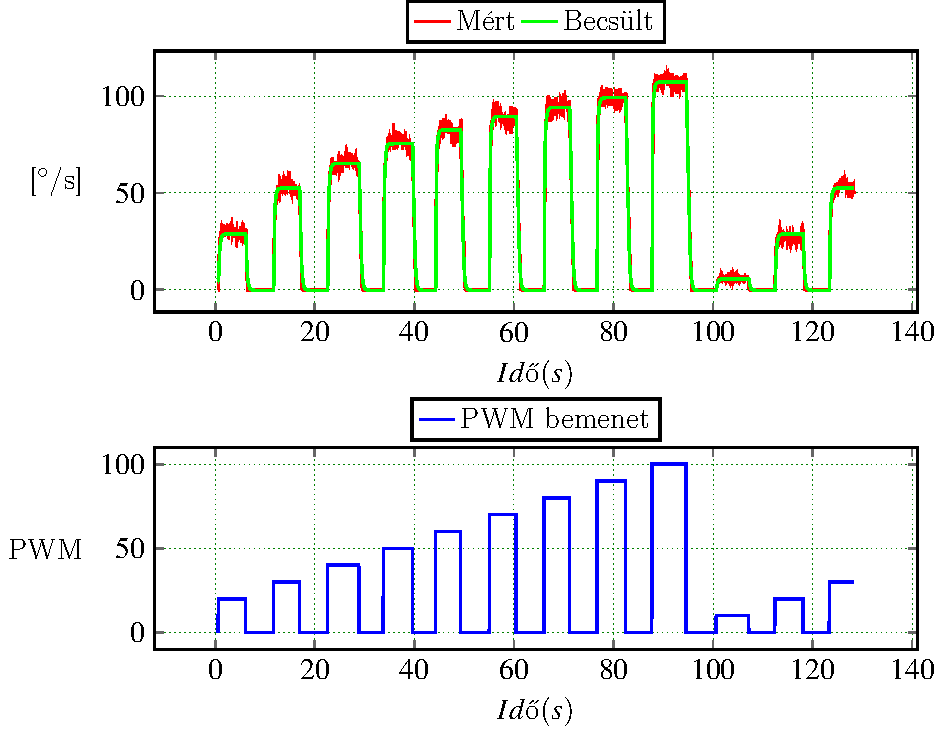
\includegraphics{tikz/NFsysIdent.pdf}
  \caption{Nagy fokozat Hammerstein-Wiener becsult model valasza, es a mert ertekek.}
  \label{fig:NFsysIdent}
\end{figure}


Az atviteli fuggveny a bemenet 50/\% korul linearizalva.

\begin{equation}
    H_s(z)=\frac{-0.07017z^{-2} -0.053z^{-1}}{-0.2117^{-3}+0.7321z^{-2} -1.393z^{-1} +1}
\end{equation}

A tervezett PID szabályozó paramétere Kp: 7.11 , Ti: 23.66 , Td: 0.43

\subsection{Kisebik fokozatban}

A becsult modelt oszehasonlitva a mert ertekekkel a \ref{fig:KFsysIdent}, a model nemlinearis becsult model megfelel a mert ertekeknek.


\begin{figure}[H]
  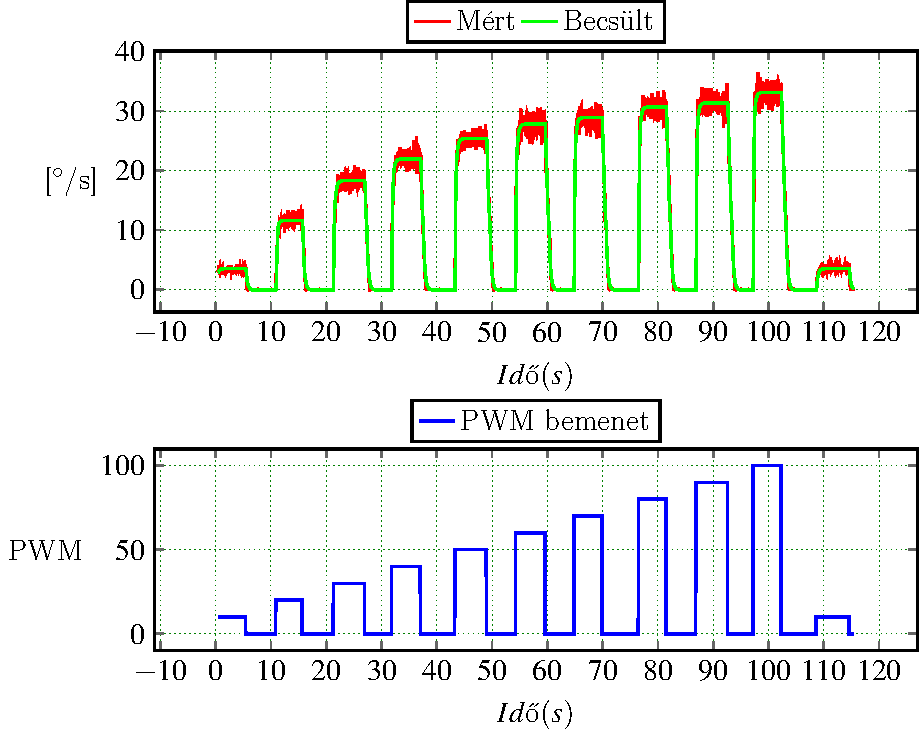
\includegraphics{tikz/KFsysIdent.pdf}
  \caption{Kis fokozat Hammerstein-Wiener becsult model valasza, es a mert ertekek.}
  \label{fig:KFsysIdent}
\end{figure}

Az atviteli fuggveny a bemenet 50/\% korul linearizalva.

\begin{equation}
    H_s(z)=\frac{-0.0291z^{-2} -0.009263z^{-1}}{-0.198z^{-3}+0.7058z^{-2} -1.394z^{-1} +1}
\end{equation}

A tervezett PID szabályozó paraméterek: Kp: 15.96 , Ti:51.51 , Td:1.237 

.



\newpage
\section{Pályakövetési feladatok}

A robot pályakövetési feladatát megfogalmazhatjuk úgy, hogy tudjunk eljutni A pontból B pontba, ha ismerjük a robot síkbeli pozícióját és az orientációját egy térképen, amely megfelel a környezetnek, látható az \ref{fig:PositionController} ábrán.
A \ref{fig:PositionController} ábrán látható, hogy felveszünk egy pozitív és egy negatív irányt a szögre nézve, az orientációkat mindig [0\degree 360\degree] között kell megadjuk. A robotnak mindig arra kell fordulnia, amerre a szög a legkisebb, azért, hogy minél kevesebbet keljen mozogjon.
A kiinduló állapotban a robot kezdetben az A pontban van és az orientációja $\beta_0$ és a B pontba szeretnénk eljutni egyenes vonalban. Így a robotnak kezdetben a célra kell fordulnia és ezután haladhat előre, miközben korrigálja az orientációs hibákat.
Első lépésben a robotnak fordulnia kell $error$ szöget, hogy $\beta_1$ irányba mutasson és ezután haladhat a cél fele.


\begin{figure}[H]
    		%trim = bal also jobb felso
   \fbox{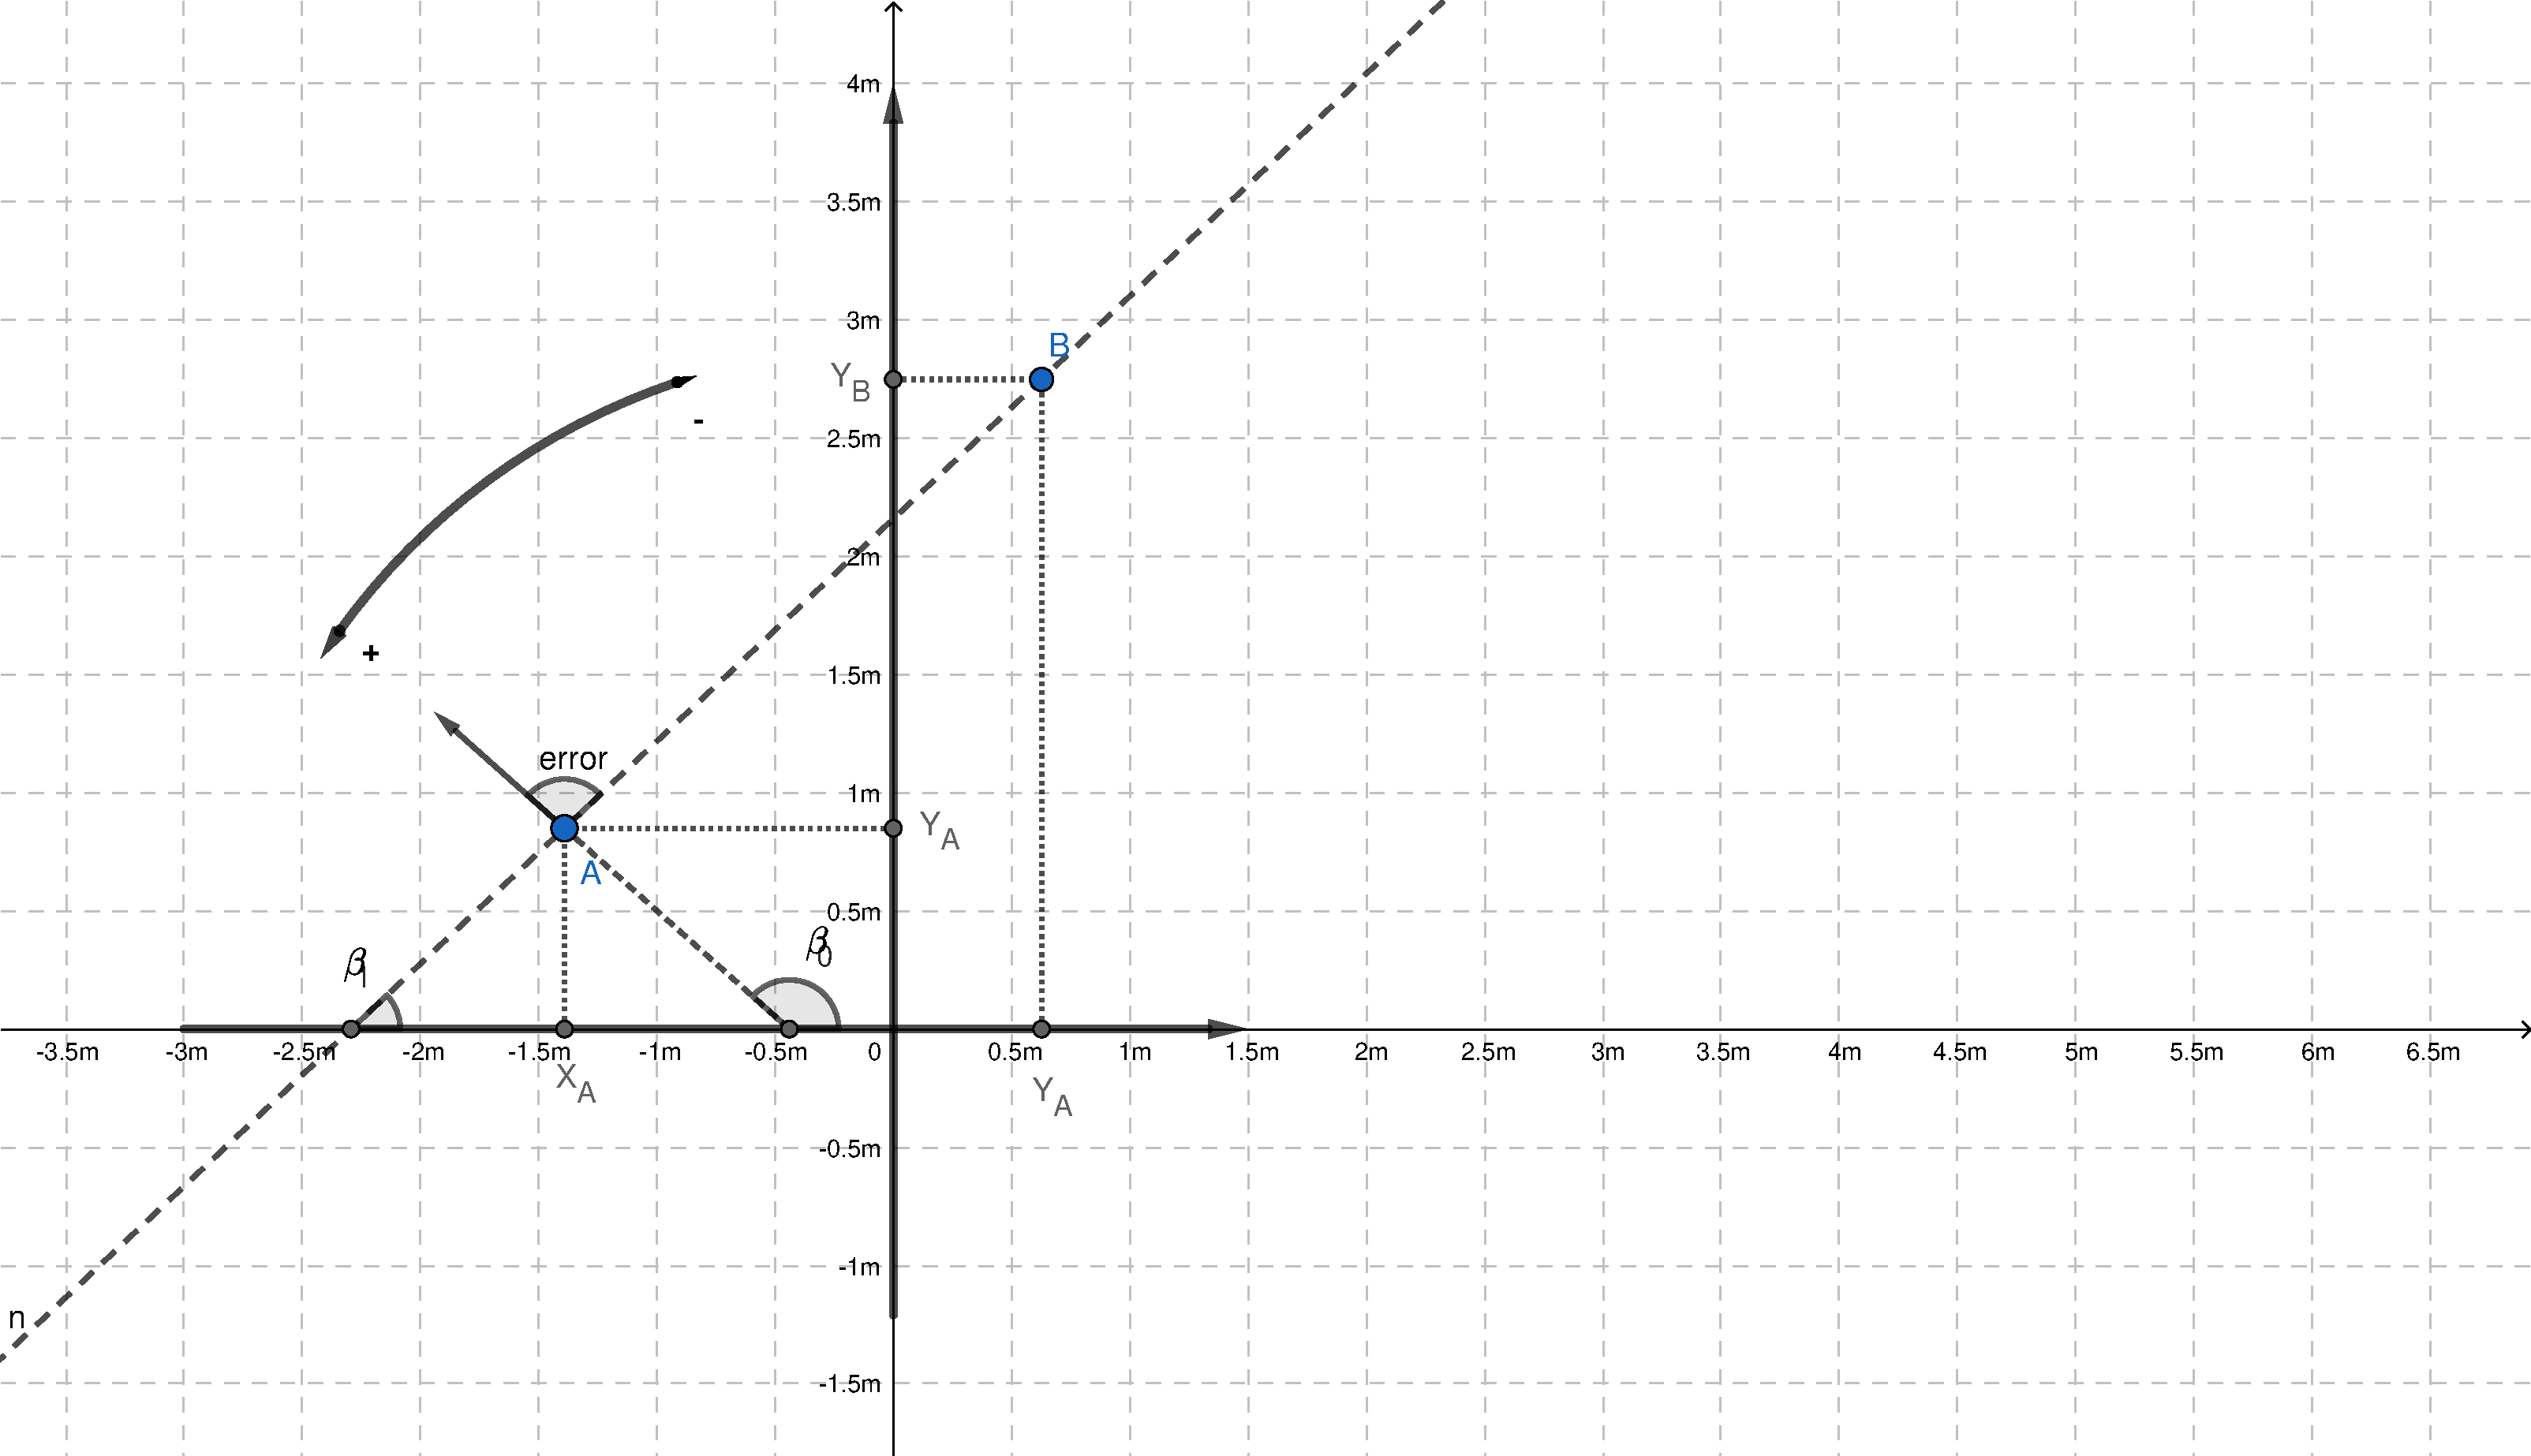
\includegraphics[width=1\columnwidth,trim=3cm 6cm 27cm 2cm,clip]{tikz/PositionController.pdf}}
  \caption{Robot pozíció szabályzása}
  \label{fig:PositionController}
\end{figure}


A pályakövetési algoritmus látható alább. Az  előírt irányt $tan^{-1}$ függvény segítségével határozzuk meg, ismerve X és Y tengelyen a hibák nagyságát. A Rotate($e_\alpha$,$\Omega_{max}$) függvényben alkalmazunk egy PI típusú szabályzót, melynek a feladata a szöghiba 0-hoz való közelítése. A Vx(d,$V_max$) a robot lineáris sebességének a szabályzását látja el egy PI típusú szabályzó, célja a robot és a kitűzött cél távolságának a csökkentése. 
A távolságszabályzó bemenetét súlyozzuk $1/e_\alpha$ értékkel, hogy ameddig nincs a robot irányban, addig ne domináljon távolságszabályzó.

\begin{algorithm}
   \caption{Pályakövetés Algoritmusa}
    \begin{algorithmic}[1]
     %\Function{GetNextControl}{$X_a,Y_a\alpha$}
      \Function{GetNextControl}{$X_a,Y_a,\alpha_a,X_t,Y_t,\alpha_t,Tr,Tr_\alpha,\Omega_{max},V_{max}$}
      %\Comment{Ahol X,Y - pozicio a térképén, \alpha irány, a - aktuális, t - előírt, Tr - pozicio hiba küszöb, $Tr_{\alpha}$ - szöghiba küszöb,${\Omega}_{max}$ maximális forgási sebesseg, $V_{max}$ maximális haladási sebesség. }
      
       \State $e_x = X_a-X_t$
       \State $e_y = Y_a-Y_t$
       \State $d=\sqrt{e_x^2+e_y^2}$
       \State $\alpha_i=dir(X_a,Y_a,X_t,Y_t)$ \Comment{Két ponton átmenő egyenes iránytényezője}
       \State $e_\alpha=\alpha_i-\alpha_a$
            \If {$e_\alpha > Tr_\alpha$} \Comment{Fordulj a cél fele}
                \State $\Omega = Rotate(e_\alpha,\Omega_{max}) $
                \State $V_x = 0 $
            \Else \Comment{Haladj a cél fele és korrigáld az elfordulást}
                
                \State $\Omega = Rotate(e_\alpha,\Omega_{max}) $
                \State $V_x = Vx(d*1/e_\alpha,V_{max})$
            \EndIf
     
            \If {$e_\alpha < Tr_\alpha$ és $d<Tr$} \Comment{Kívánt pozícióban}
                \State $\Omega = 0$
                \State $V_x = 0 $
            \EndIf
        
       \EndFunction

\end{algorithmic}
\end{algorithm}



Az algoritmus tesztelésére MATLAB/Simulink környezetet használtam. A robot kinematikai modellt az \ref{eq:allapot} egyenlet alapján modelleztem, a pozíciók (X,Y) és az irány meghatározására integráltam a lineáris és szögsebességeket. 

A \ref{fig:SimPoseCont} ábrán láthatjuk a szimulációs eredményeket, amint a robot egy végtelen jelhez hasonló pályát követ.

\begin{figure}[H]
	\setlength{\fboxsep}{0pt}
	\setlength{\fboxrule}{0pt}
	
    \begin{center}  	
    		%trim = bal also jobb felso
    	\fbox{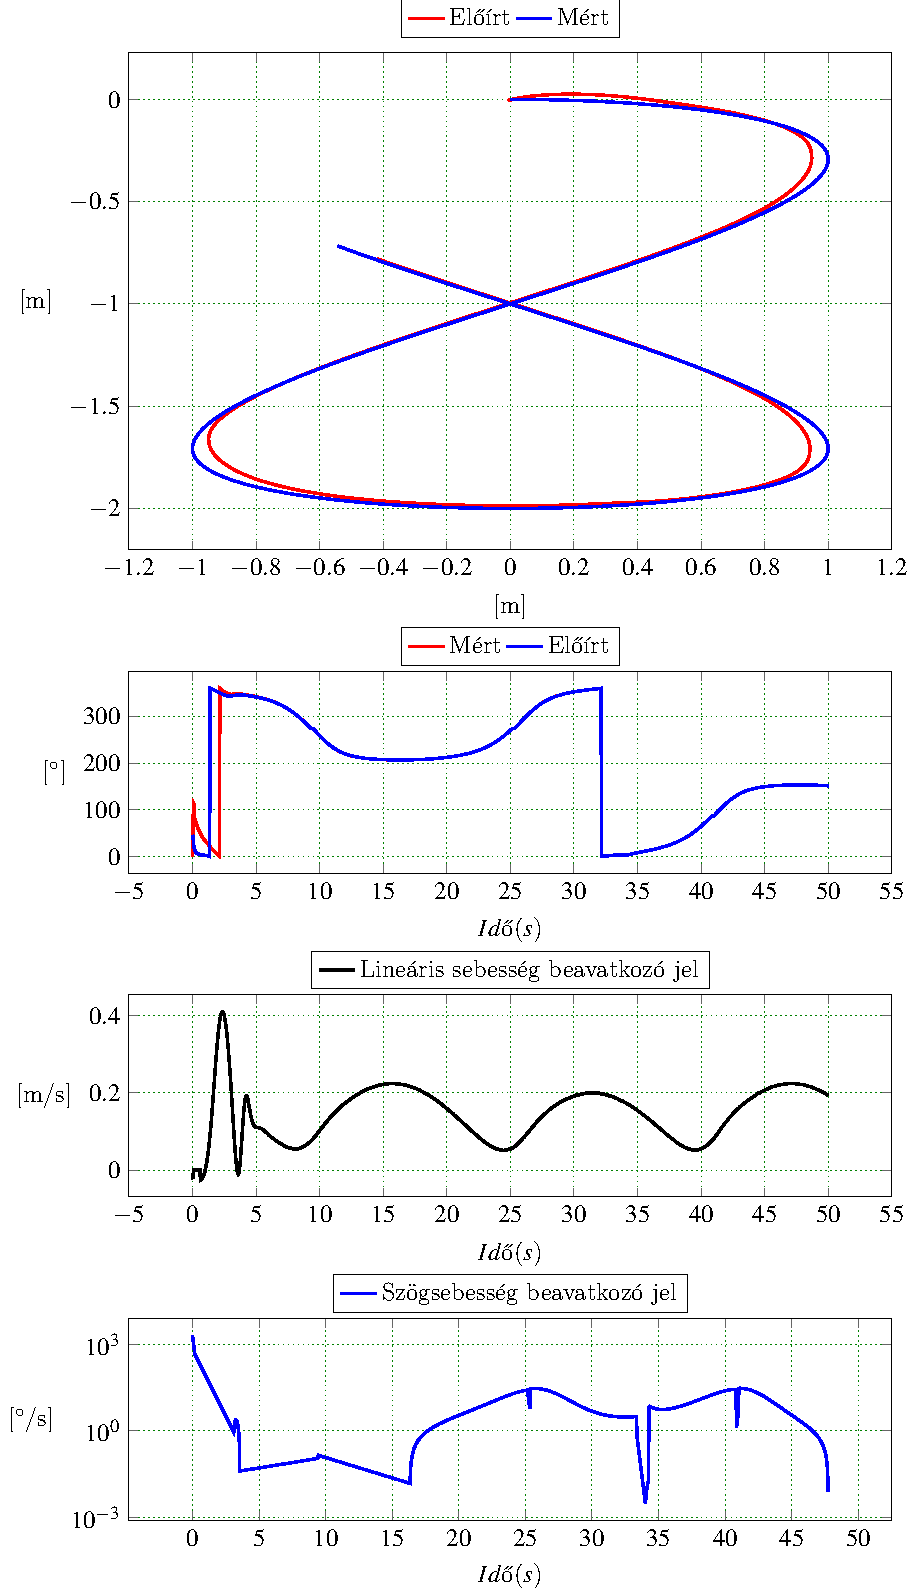
\includegraphics[width=0.9\columnwidth,trim=0cm 0cm 0cm 0cm,clip]{tikz/SimPoseCont.pdf}}
    \end{center}  
    
  	\caption{Robot pozíció szabályzása}
  	\label{fig:SimPoseCont}
\end{figure}

